\chapter{Desarrollo de herramientas bioinformáticas para el análisis de duplicidades genéticas}
\label{chapter: desarrollo}

% En estos capítulos, hay que describir los aspectos más relevante del diseño y desarrollo del proyecto, así como de los productos obtenidos. La estructuración de los capítulos puede variar según el tipo de Trabajo.  

% En cada apartado es muy importante describir las alternativas posibles, los criterios utilizados para tomar decisiones y la decisión tomada.

% En caso de que corresponda, se incluirá un apartado de “Valoración económica del trabajo”. Este apartado indicará los gastos asociados al desarrollo y mantenimiento del trabajo, así como los beneficios económicos obtenidos. Hacer un análisis final sobre la viabilidad del producto.


%% añadir una primera fase que resuma todo

%% Ejemplo:
Para poder realizar una búsqueda de genes duplicados contenidos en un genoma se requiere obtener la información tanto de la anotación como de la secuencia proteica de cada gen codificante. Para ello es necesario un preprocesado de la información contenida en los diferentes ficheros de anotación y una posterior búsqueda de secuencias duplicadas. Posteriormente se representa toda esta información generada en un gráfico que muestre las relaciones entre las duplicaciones encontradas y su situación dentro del genoma.

A continuación se detalla cada fase del proceso y el desarrollo de las herramientas creadas para realizar cada tarea. Todo el código generado y la documentación necesaria para replicar el trabajo hecho se puede encontrar en el siguiente repositorio de github:

************************ link github

%% hacer referencia al github y poner link



En la figura \ref{fig:workflow} se muestran los pasos del proceso de análisis desde la entrada de información hasta la generación resultados y gráficos.

\begin{figure}[h]
	\centering
	\captionsetup{width=\linewidth} 
	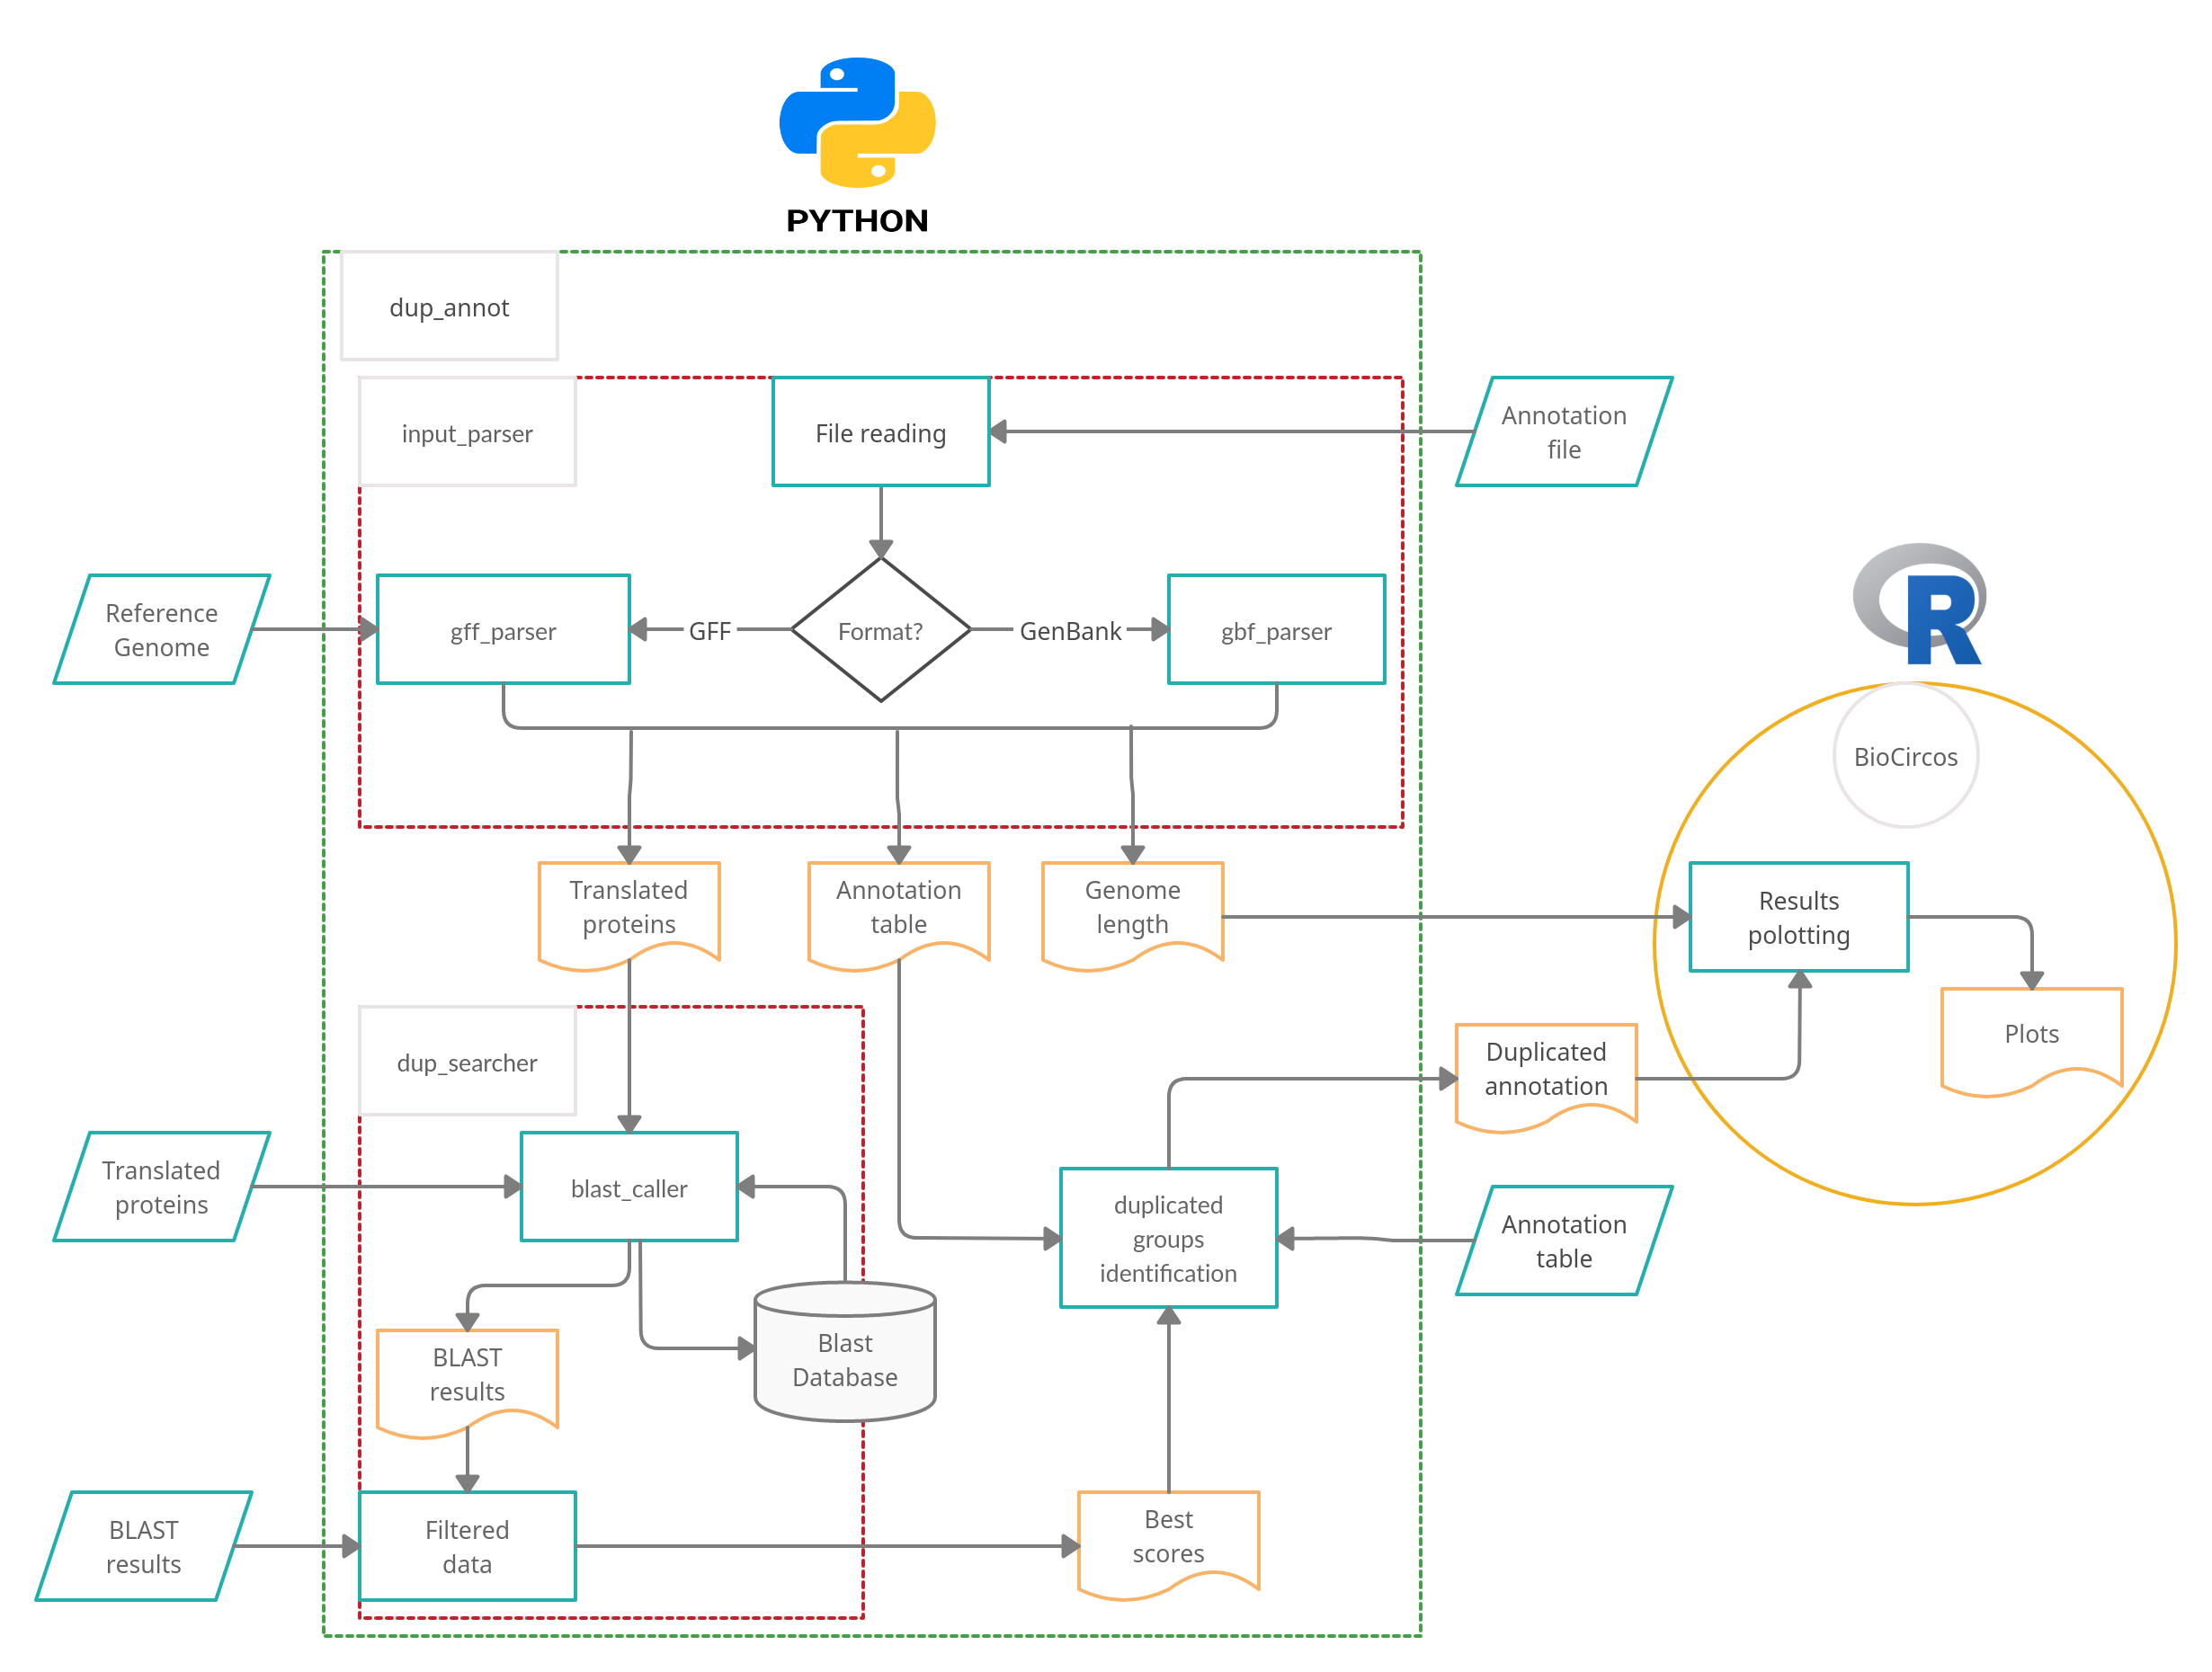
\includegraphics[width=\linewidth]{figs/workflow.png}
	\caption[Diagrama de flujo de datos de los programas desarrollados]{Diagrama de flujo de datos de los programas desarrollados donde puede seguirse el recorrido de los datos desde que entran en el programa hasta que se generan los resultados. Los paralelogramos corresponden a entrada de información desde el exterior (usuario); los rectángulos identifican cada función en python que desarrolla el proceso; las líneas de puntos engloban los módulos que contienen las correspondientes funciones en python; los círculos engloban los procesos desarrollados en R.}
	\label{fig:workflow}
\end{figure}

\section{Módulos en $python$}

\subsection{Requerimientos}

% añadido
El objetivo de este proyecto es comenzar el desarrollo de un paquete de python que permita la generación de análisis de duplicaciones a partir de ficheros de anotación. Para el desarrollo y testado de este paquete se ha utilizado la versión 3.8.5 de python y creado un entorno virtual específico para el TFM con el siguiente comando:

%% dejar espacio

%% a mi personalmente me gusta mas en gris que en negro 
% pues que se haga el gris

\vspace{5mm}

\colorbox{gray}{\textcolor{white}{\$ mkdir environments}}

\colorbox{gray}{\textcolor{white}{\$ cd environments}}

\colorbox{gray}{\textcolor{white}{\$ python3 -m venv TFM}}    

\vspace{5mm} %% espacio

Seguidamente, se instala el paquete de instalación $pip$ que nos permitirá descargar módulos específicos necesarios para el funcionamiento de nuestro programa.

\vspace{3mm}
\colorbox{gray}{\textcolor{white}{\$ sudo apt install -y python3-pip}}
\vspace{3mm}

En el apéndice \ref{apA} se facilita la lista de módulos instalados a lo largo del desarrollo del programa y una breve descripción de los módulos instalados con $pip$.

%% añadido
Para la generación de búsquedas de similitud de secuencias, necesitamos hacer uso de BLAST+, en concreto de la herramienta Blastp, la cual compara secuencias de proteína a estudio con una base de datos de proteínas de referencia \cite{bethesda_md_national_library_of_medicine_us_blast_nodate,altschul_basic_1990}. En el apéndice \ref{apA} se muestra su instalación y funcionamiento desde el terminal \cite{bethesda_md_national_center_for_biotechnology_information_us_blast_2008}.

\subsection{Entrada de datos e información}

La información proporcionada por el usuario puede ser de diferentes tipos y presentarse en diferentes formatos:

\begin{itemize}
\item \textbf{Anotación y ensamblaje de un genoma:} Pueden provenir de una base de datos RefSeq o GenBank como la de \textit{National Center for Biotechnology Information} (NCBI) \cite{national_center_for_biotechnology_information_national_1988} o haber sido ensambladas \textit{de novo}. Nuestro programa admitirá dos tipos de formatos que incluyan la anotación del genoma:  \href{https://www.ncbi.nlm.nih.gov/Sitemap/samplerecord.html}{GenBank} y \href{https://www.ncbi.nlm.nih.gov/Sitemap/samplerecord.html}{GFF3}, este último deberá ir acompañado de un archivo \href{https://blast.ncbi.nlm.nih.gov/Blast.cgi?CMD=Web&PAGE_TYPE=BlastDocs&DOC_TYPE=BlastHelp}{fasta} que contenga la secuencia genómica de referencia correspondiente mientras que los archivos en formato GenBank, ya tienen incluida esta información al final del documento.

\item \textbf{Proteínas de interés:} Archivo en formato fasta con las proteínas traducidas. Pueden provenir de trabajos previos. Deben ir acompañadas de un archivo $csv$ con la anotación del genoma.
\item \textbf{Tabla de anotación:} Archivo en formato $csv$ en el que aparezca la anotación del genoma a estudio. Debe ir acompañado de un archivo fasta con las secuencias proteicas.
\end{itemize}

Dependiendo del tipo de información, el tratamiento de la misma será diferente.

\subsection{Tratamiento de datos de anotación: input\_parser.py}

Como se puede apreciar en la figura \ref{fig:usage_input_parser}, el módulo input\_parser.py se define con una serie de argumentos necesarios para activar el proceso. En caso de no proporcionar aquellos obligatorios (archivo de anotación y carpeta de salida donde se guarden los archivos generados) se generará un error que no permitirá continuar (Figura \ref{fig:error_input_parser}). 


\begin{figure}[h]
\centering
    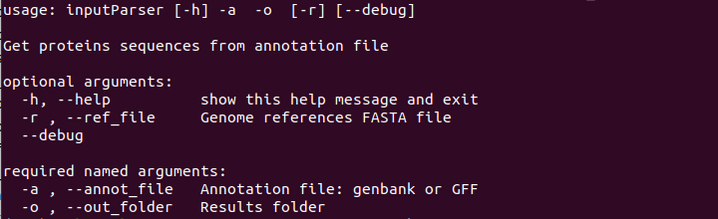
\includegraphics[width=0.7\textwidth]{figs/usage_input_parser.png}
    \caption[Información del uso de input\parser en la terminal]{Información del uso de argumentos de input\_parser.}
    \label{fig:usage_input_parser}
\end{figure}


Este módulo se encarga. en primer lugar, de tomar los ficheros de entrada y determinar su formato. En función de la extensión del archivo, llamará a la función que analiza archivos GFF o GenBank. Si la extensión no se incluye dentro de un listado determinado, se generará un error y el programa no continuará el proceso. 

\begin{figure}[h]
	\centering
	\captionsetup{width=0.7\linewidth} 
	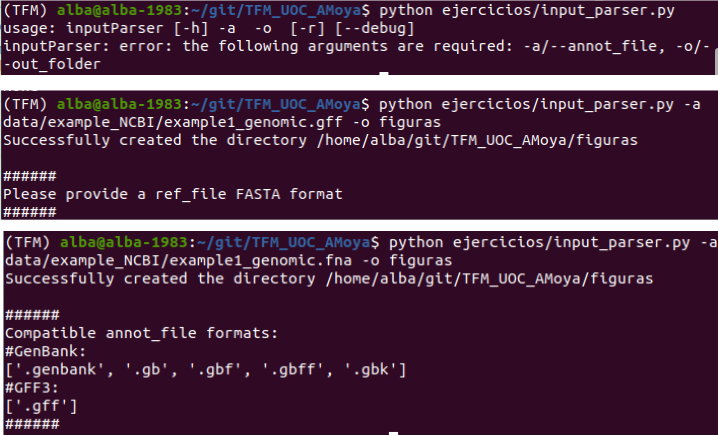
\includegraphics[width=0.7\linewidth]{figs/error_input_parser.png}
	\caption[Errores en input\_parser.py]{Diferentes errores que pueden ocurrir: Falta de carpeta de salida (arriba) o de archivo de referencia genómica (centro) y formato incorrecto (abajo).}
	\label{fig:error_input_parser}
\end{figure}

%% Añadido
Puesto que la información contenida en cada tipo de fichero de anotación esta estructurada de forma diferente el manejo de esta debe ser acorde a sus características. Si tenemos un archivo GenBank, se llamará a \textbf{gbf\_parser.py} para que lleve a cabo la conversión de los datos a las secuencias de proteínas traducidas. Además, generará un fichero de texto plano con la información contenida en el archivo de anotación en forma de tabla. Si, en cambio, tenemos un archivo GFF, se invocará a \textbf{gff\_parser.py}, el cual necesitará que también se facilite el archivo de referencia genómica para poder producir el archivo de proteínas. Si este segundo archivo no se proporciona, el programa detectará un error y no continuará el proceso (Figura \ref{fig:error_input_parser}).


Al terminar el proceso, obtendremos una carpeta de salida con tres documentos:

\begin{itemize}
\item df.csv: tabla de anotación del genoma que se utilizará (Figura \ref{fig:annot_table}). Está formada por 13 columnas de anotación que describen a cada una de las id únicas (protID) generadas por el programa para cada entrada. 

\begin{figure}[h]
	\centering
	\captionsetup{width=\linewidth} 
	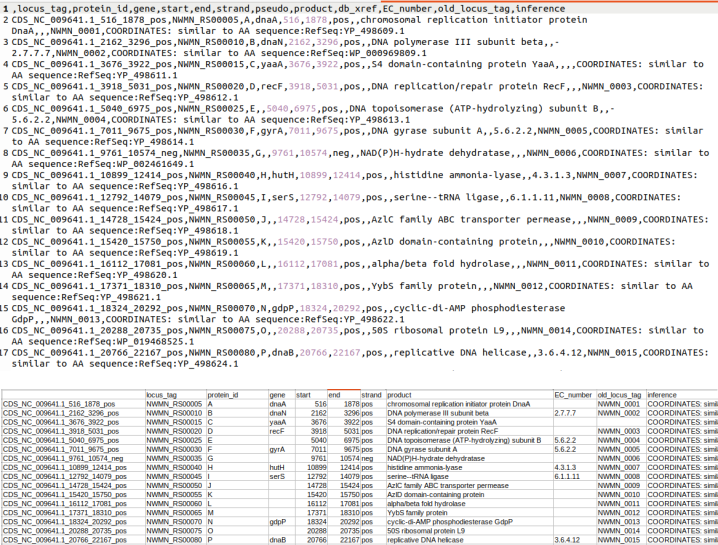
\includegraphics[width=\linewidth]{figs/annot_table.png}
	\caption[Tabla de anotación del genoma]{Tabla de anotación generada tras el tratamiento de los datos con input\_parser.py.}
	\label{fig:annot_table}
\end{figure}


\item proteins.fa: archivo en formato fasta con las secuencias proteicas provenientes de la traducción de las diferentes regiones de codificación del genoma (CDS)
\item length.csv: tabla en la que se incluye los diferentes identificadores de secuencia contenidos en los archivos de anotación proporcionados y su tamaño en pares de bases (pb).
\end{itemize}

\subsection{Comparación de secuencias con BLAST+: blast\_caller.py}
%% pequeña introductocción de que hace
BLAST+ (\textit{Basic Local Alignment Search Tool}) es una herramienta informática de alineamiento de secuencias. Puede realizar búsquedas en las bases de datos de secuencias en cuestión de segundos para encontrar similiritudes con las secuencias problema alineándolas por pares. Hay cinco variantes del algoritmo dependiendo del tipo de secuencias que se comparen entre sí: blastp para comparaciones entre proteínas; blastn compara secuecias de nucleótidos; blastx y y tblastn entre las posibles traducciones de secuencias de nucleótidos y bases de datos de proteínas y tblastx compara las seis traduciones posibles en sus marcos de lectura de la secuencia problema contra la seis de las secuencias de la base de datos de nucleótidos \cite{madden_blast_2003, altschul_basic_1990}.

Como se ha comentado al inicio del capítulo, utilizaremos la herramienta Blastp a nivel local. Es decir, invocaremos al algoritmo con los parámetros adecuados para que utilice como bases de datos las mismas secuencias de proteínas con las que después tratará de encontrar los mejores alineamientos. Cada uno de estos alineamientos obtendrá una puntuación de calidad que indicarán el grado de similitud de las dos secuencias comparadas \cite{madden_blast_2003, altschul_basic_1990}.
%% explicar que se hace una busqueda de las propias proteinas consigo mismas para buscar duplicados internamente

El módulo blast\_caller.py se divide en dos fases:

\begin{itemize}
\item \textbf {Generación de la base de datos} local a partir del archivo de proteínas generado anteriormente.
\item \textbf {Generación resultados BLAST} comparando las secuencias de la base de datos con el mismo archivo de proteínas (las secuencias se comparan entre sí mismas dos a dos).
\end{itemize}

Este módulo se define con los argumentos requeridos y opcionales mostrados en la figura \ref{fig:usage_blast_caller}. Es necesario que el usuario aporte un archivo fasta de proteínas para que el programa funcione. Además, se debe añadir la ruta donde se encuentran los archivos ejecutables de BLAST para que puedan ser utilizados.

\begin{figure}[h]
\centering
    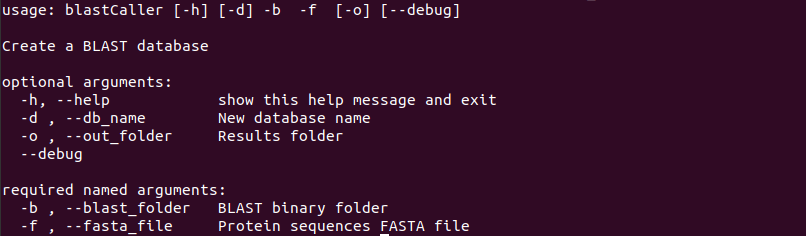
\includegraphics[width=0.7\textwidth]{figs/usage_blast_caller.png}
    \caption[Información de blast\_caller en la terminal]{Información del uso de argumentos de blast\_caller}
    \label{fig:usage_blast_caller}
\end{figure}

%% modificado
El programa permite generar el comando necesario para ejecutar BLAST+ haciendo una llamada al sistema utilizando la funcion \textit{system} de python (Figura \ref{fig:blast_caller}).

\begin{figure}[h]
	\centering
	\captionsetup{width=0.7\linewidth} 
	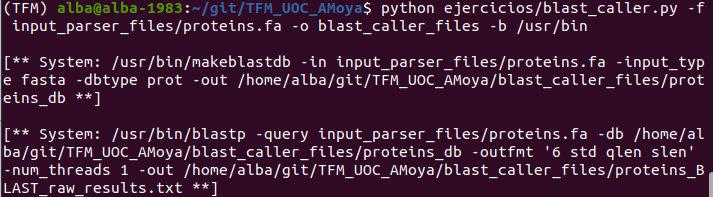
\includegraphics[width=0.7\linewidth]{figs/blast_caller.png}
	\caption[Linea de comandos blast]{Linea de comandos en la terminal para ejecutar makeblastdb y blastp}
	\label{fig:blast_caller}
\end{figure}

Al finalizar el proceso, por un lado, se obtienen tres archivos proteins\_db que forman la base de datos de proteínas, donde las extensiones \textit{phr}, \textit{pin} y \textit{psq} corresponden a las cabeceras, índices y secuencias, respectivamente. 

Por otro lado, obtenemos un fichero de con los resultados BLAST en bruto de las secuencias similares obtenidas (hits). Este último documento se presenta como una tabla con las siguientes columnas \cite{scholz_blastn_nodate, scholz_e-value_nodate}:

- id de la secuencia problema

- id de la secuencia de referencia

- porcentaje de coincidencias idénticas

- longitud del alineamiento

- número de no concordancias 

- número de huecos

- comienzo del alineamiento en la secuencia problema

- final del alineamiento en la secuencia problema

- comienzo del alineamiento en la secuencia de referencia

- comienzo del alineamiento en la secuencia de referencia

-  e-valor: número de hits de igual calidad que se espera encontrar debido al azar. Los resultados aparecen ordenados por defecto según su e-valor, los mejores hits (valores más bajos) aparecen primero. Por defecto, se establece en un valor de 10, por encima del cual los alineamientos no se incluyen en el documento.

- bit-score: tamaño de una base de datos requerido para encontrar el mismo número de concordancia por azar. Las secuencias presentan mayor similitud cuanto mayor sea su bit-score.

- longitud de la secuencia problema

- longitud de la secuencia de referencia

\subsection{Búsqueda de duplicados: dup\_searcher.py}

Este módulo ofrece dos posibilidades de datos de entrada. El usuario puede proporcionar el archivo fasta de proteínas, que hará que el módulo conecte con blast\_caller para generar el documento de resultados. O bien, puede proporcionar directamente un documento de resultados BLAST creado previamente.

Los argumentos definidos para dup\_searcher (figura \ref{fig:usage_dup_sarcher}) nos permite cambiar las variables de filtrado de los datos para generar unos resultados más o menos afinados.
Así, podemos cambiar los valores mínimos de bit-score, e-valor o los porcentajes de alineamiento o similitud, por debajo de los cuales serán eliminados de la lista de resultados. Paralelamente, se filtran las parejas espejo (cuando A=B y B=A) y las que correspondan a una secuencia alineada consigo misma (A=A). Por defecto, se ha diseñado el programa para trabajar con un e-valor $=10^{-05}$ (un e-valor bajo nos permitirá tener pocos resultados pero de buena calidad), bit-score = 50 y unos porcentajes de alineamiento y similitud del 85\%.

\begin{figure}[h]
\centering
    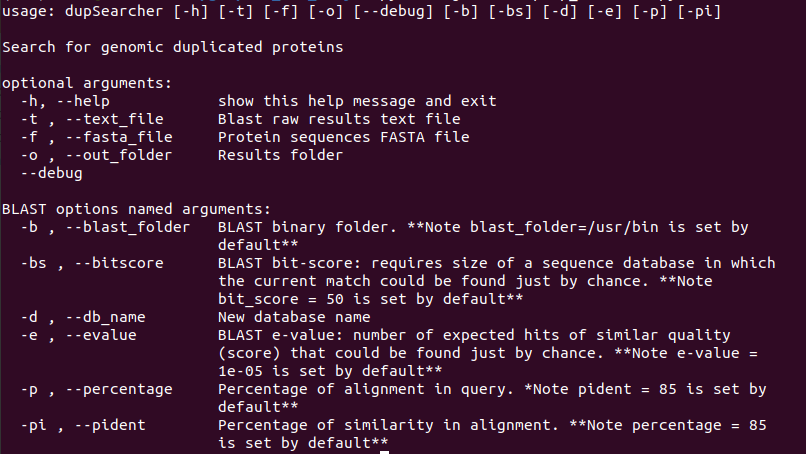
\includegraphics[width=0.7\textwidth]{figs/usage_dup_searcher.png}
    \caption[Información de dup\_searcher en la terminal]{Información del uso de argumentos de dup\_searcher}
    \label{fig:usage_dup_sarcher}
\end{figure}


El resultado final es una tabla ordenada según el porcentaje de alineamiento en primer lugar, seguido por un orden ascendente de  e-valor (los mejores resultados, e-valor menor, primero) y bitscore en sentido descendente. Añadimos los encabezados de las columnas y obtenemos un documento similar a la figura \ref{fig:dup_annot}

\begin{figure}[h]
	\centering
	\captionsetup{width=\linewidth} 
	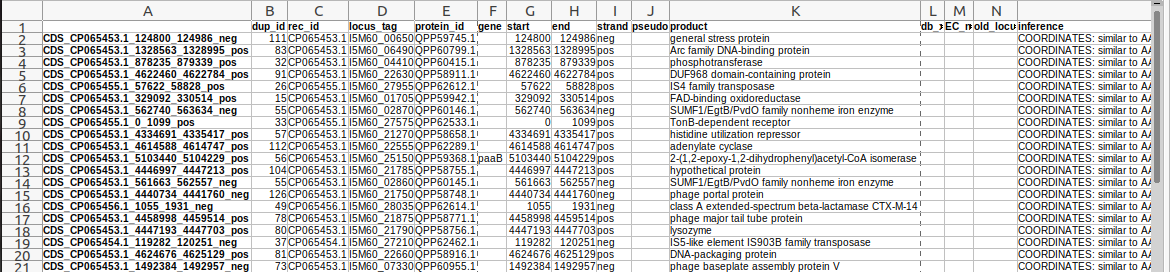
\includegraphics[width=\linewidth]{figs/dup_annot.png}
	\caption[Tabla de anotación del genoma]{Tabla de anotación generada tras el tratamiento de los datos con input\_parser.py}
	\label{fig:dup_annot}
\end{figure}


\subsection{Anotación de las proteínas duplicadas: dup\_annot.py}
Este módulo engloba a todos los anteriores. Los argumentos definidos (figura \ref{fig:usage_dup_annot}) lo dotan de la flexibilidad necesaria para generar los resultados independientemente del tipo de información proporcionada, iniciando el proceso a partir del punto correspondiente según la misma.

\begin{figure}[h]
\centering
    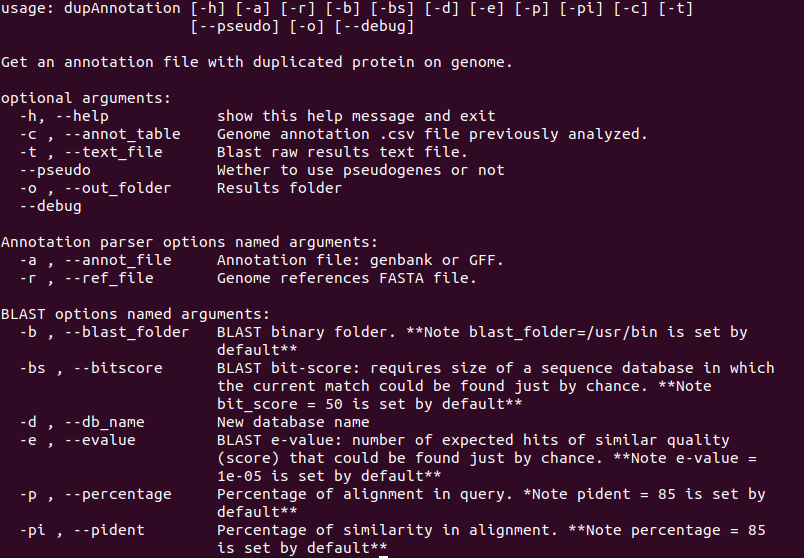
\includegraphics[width=0.7\textwidth]{figs/usage_dup_annot.png}
    \caption[Información de dup\_annot en la terminal]{Información del uso de argumentos de dup\_annot}
    \label{fig:usage_dup_annot}
\end{figure}



Además de los argumentos incluidos en los módulos anteriores, añadimos uno nuevo que permitirá elegir si se quiere tener en cuenta los pseudogenes o no en el resultado final.

El módulo dup\_annot.py toma los resultados en bruto de BLAST e identifica los diferentes grupos de duplicados, teniendo en cuenta que si A=B y B=C, entonces A=B=C. Esta nueva información la volcará en la tabla de anotación generada en input\_parser (o proporcionada por el usuario), de la cual se mantendrán únicamente las proteínas duplicadas.  De esta forma, obtenemos una tabla de anotación completa para cada una de las proteínas duplicadas, identificadas por el grupo de duplicado al que pertenecen.

Al finalizar el proceso, el programa muestra en pantalla cuántos grupos y proteínas duplicadas ha encontrado con los parámetros de BLAST introducidos (figura \ref{fig:salida_dup_annot})

\begin{figure}[h]
	\centering
	\captionsetup{width=0.7\linewidth} 
	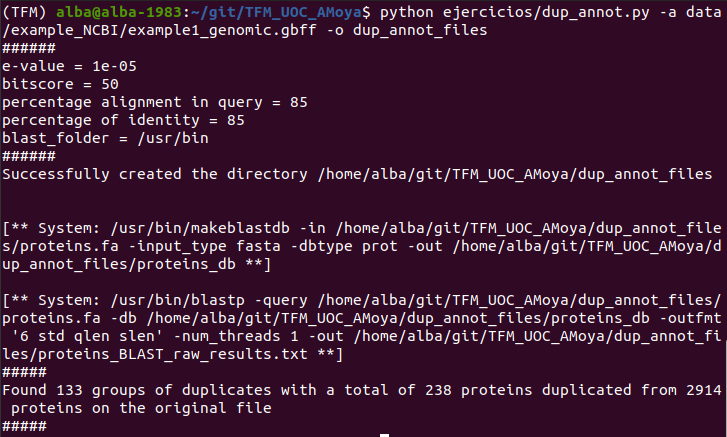
\includegraphics[width=0.7\linewidth]{figs/salida_dup_annot.png}
	\caption[Mensaje terminal de dup\_annot.py]{Mensaje mostrado en la terminal de Linux al terminar el proceso de dup\_annot.py.}
	\label{fig:salida_dup_annot}
\end{figure}

\subsection{Archivos obtenidos} 

Como muestra la figura (\ref{fig:salida_dup_annot}) al final del proceso obtenemos una carpeta con todos los archivos generados juntos.

\begin{figure}[h]
	\centering
	\captionsetup{width=0.4\linewidth} 
	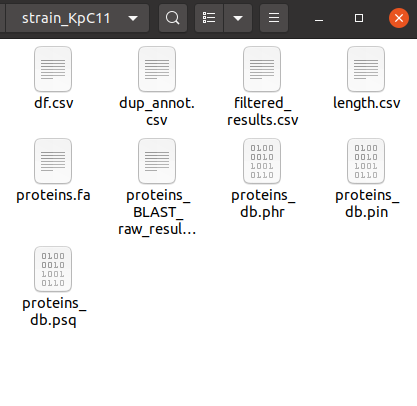
\includegraphics[width=0.4\linewidth]{figs/input_parser_files.png}
	\caption[Carpeta de resultados]{Carpeta de resultados generada tras ejecutar el programa dup\_annot.py}
	\label{fig:salida_dup_annot}
\end{figure}

- Del tratamiento de datos con input\_parser se obtienen los archivos df.csv (tabla de anotación completa), proteins.fa (secuencias de proteínas) y length.csv (longitudes de los diferentes genomas contenidos).

- La búsqueda de resultados con dup\_searcher nos proporciona los archivos pertenecientes a la base de datos creada (proteins\_db), el archivo proteins\_BLAST\_raw\_resuts.txt con los alineamientos generados y filtered\_results.csv tras pasar por el proceso de filtrado de los mejores resultados.

- Finalmente, dup\_annot.csv es la tabla de anotación para las proteínas identificadas como duplicados.

\section{Módulo en $\mathbb{R}$}

Se ha utilizado la versión 4.0.3 de R, en el entorno de desarrollo RStudio (versión 1.3.1073). Se ha creado un proyecto específico para desarrollar el paquete cuyas especificaciones se detallan en el apéndice \ref{apA}.

Se ha utilizado el paquete \textbf{BioCircos} \cite{cui_biocircosjs_2016, vulliard_biocircos_2019} para generar gráficos circulares que representen el cromosoma bacteriano y sus posibles plásmidos, resaltando los genes duplicados y sus grupos localizados en la primera fase del proyecto. En la figura \ref{fig:ex_BioCircos} se puede ver un ejemplo de gráfico generado con BioCircos.

\begin{figure}[h]
	\centering
	\captionsetup{width=0.5\linewidth} 
	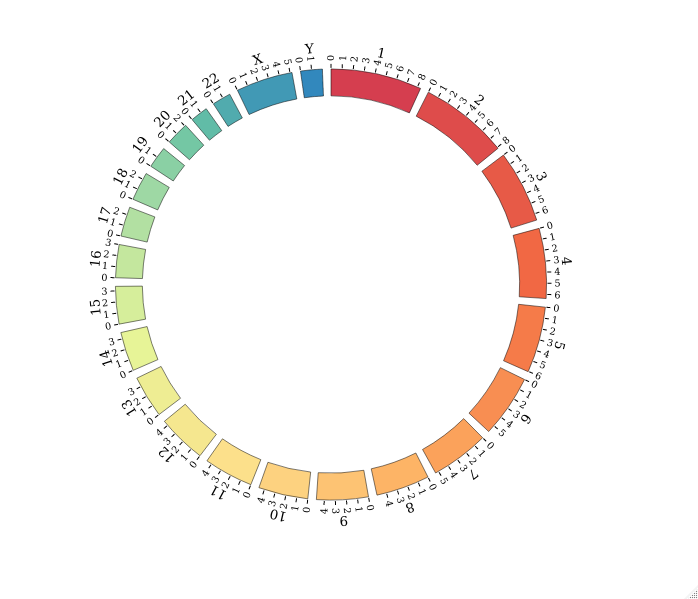
\includegraphics[width=0.5\linewidth]{figs/ex_biocircos.png}
	\caption[Ejemplo de gráfico BioCircos]{Gráfico generado automáticamente con los datos por defecto del paquete BioCircos de R. Se pueden ver los diferentes cromosomas del genoma humano identificados por colores y con un tamaño proporcional con respecto a la totalidad del genoma.}
	\label{fig:ex_BioCircos}
\end{figure}

A continuación se hará una breve descripción de las funciones más significativas del módulo. 

\begin{itemize}
    \item \textbf{duplicate\_group\_tracks:} para cada grupo de duplicados se determinará el cromosoma o plásmido a los que pertenecen sus componentes (rec\_id), posición e inicio de cada secuencia. Se generará un \textit{track} en el que las secuencias duplicadas se conectaran con líneas con los miembros de su grupo de duplicación.
    \item \textbf{parse\_data}: genera la información que se mostrará al pasar el cursor del ratón por encima de cada secuencia duplicada y la paleta de colores que identificará cada tipo de información.
    \item \textbf{add\_genes\_strand:} para cada hebra del cromosoma, se creará un círculo o track donde se podrán ver los genes duplicados alojados.
    \item \textbf{create\_BioCircos:} finalmente se crea el gráfico con la información generada en las funciones previas.
\end{itemize}

%% añade un ejemplo bonito de biocircos con tus datos y lo comentas brevemente sin entrar en detalle de los resultados.